\documentclass[amsmath,amssymb,twocolumn,superscriptaddress]{revtex4-1}

\usepackage{graphicx}% Include figure files
\usepackage{dcolumn}% Align table columns on decimal point
\usepackage{bm}% bold math
\usepackage[detect-all]{siunitx}
\usepackage{hyperref}% add hypertext capabilities
\usepackage{xr}

\begin{document}                  % DO NOT DELETE THIS LINE

\title{Introducing classical molecular dynamics simulation to users of
scattering}

\author{A.~R. McCluskey}
\email{a.r.mccluskey@bath.ac.uk}
\affiliation{Department of Chemistry, University of Bath, Claverton Down,
Bath, BA2 7AY, UK}
\affiliation{Diamond Light Source, Harwell Campus, Didcot, OX11 0DE, UK}

\author{A.~R. Symington}
\affiliation{Department of Chemistry, University of Bath, Claverton Down,
Bath, BA2 7AY, UK}

\author{J. F. T. B. Snow}
\affiliation{Diamond Light Source, Harwell Campus, Didcot, OX11 0DE, UK}
\affiliation{School of Chemistry, University of Bristol, Bristol, BS8 1TS, UK}

\author{J. Grant}
\affiliation{Computing Services, University of Bath, Claverton Down, Bath, BA2 7AY, UK}

\author{B.~J. Morgan}
\affiliation{Department of Chemistry, University of Bath, Claverton Down,
Bath, BA2 7AY, UK}

\author{S.~C. Parker}
\affiliation{Department of Chemistry, University of Bath, Claverton Down,
Bath, BA2 7AY, UK}

\author{K.~J. Edler}
\email{k.edler@bath.ac.uk}
\affiliation{Department of Chemistry, University of Bath, Claverton Down,
Bath, BA2 7AY, UK}

\date{\today}

\begin{abstract}
Classical molecular dynamics simulations are becoming a popular technique for the multi-modal analysis of scattering techniques; such as small angle scattering and diffraction.
However, few users of these techniques have formalised training in these methodologies, resulting in frequent use of molecular dynamics simulations as a black box technique.
This work discusses an open educational resource designed to introduce classical molecular dynamics to users of scattering, describing possible sources of error in the method.
Furthermore, we cover some of the methods that can be used to enable simulation techniques to facilitate in the analysis of scattering data.
\end{abstract}

\maketitle                        % DO NOT DELETE THIS LINE

\section{Introduction}

The use of molecular dynamics simulations to aid in the analysis of experimental data; particular from small angle scattering and diffraction, has grown significantly over the past ten years \cite{Pan2012,Boldon2015,Hub2018,Ivanovic2018,East2016,Wall2014,Wall2018,Satoh2015}.
Figure \ref{fig:growth} shows the growth in the percentage of small angle scattering (SAS) publications that mention molecular dynamics.
It can be seen that there has been a linear growth in such publications, with more than \SI{20}{\percent} of all SAS publications mentioning molecular dynamics as of 2018.
This alone is a clear indication of the importance simulation techniques are having on the field of scattering and diffraction.

Normally, the users of scattering and diffraction techniques have a background in experimental science, with little or no formalised training in computational modelling techniques.
This may be problematic, as it can lead to the use of molecular simulation as a black-box, with little understanding or consideration for the underlying methodologies.
The use of molecular simulation in this fashion can quickly lead to the inclusion of severe, systematic errors.
This has lead to the development of tools, such as WAXSiS or SASSIE \cite{Chen2014,Knight2015,Perkins2016}, that present easy-to-use interfaces designed to reduce the risk of these errors.

In addition to the development of software packages, another method to further limit systematic errors, are lectures or courses presenting and introduction to molecular simulation for scattering and diffraction users.
For example, the annual ISIS Neutron Training Course now included an ``Introduction to Molecular Dyanmics for Neutron Scattering'' module.
This details the fundemental of classical molecular dynamics simulation, before presenting some previous applications of these methods in neutron science and allowing the students to gain a familiarity with the SASSIE package.
While such courses and modules are an important aspect of training, they are limited both in numbers of students that may attend and location, meaning that not scattering and diffraction users may easily access them.
%
\begin{figure}
\label{fig:growth}
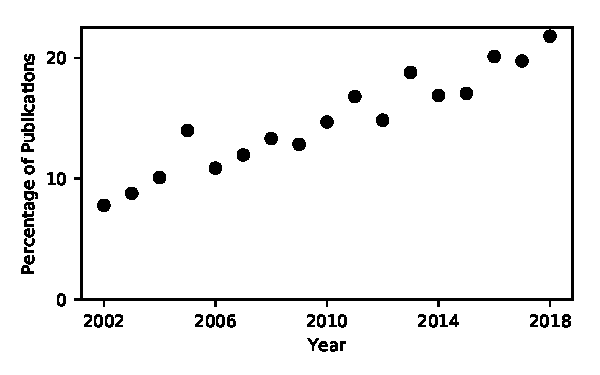
\includegraphics[width=0.48\textwidth]{figures/chem_data_py.pdf}
\caption{The annual growth of the percentage of publication that mention ``small angle scattering'' which also mention ``molecular dynamics. Determined from the number of results from a Google Scholar search.}
\end{figure}
%

There has been a recent movement within the scientific and engineering communities towards technology-enchanced open educational resources (OERs).
These are courses, lectures, or learning modules that are made free available online for use by anyone.
This allows the permission for others to engage in the ``5R activities'': Retain, Reuse, Revise, Remix, and Redistribute \cite{opencontent2018}.
The act of publishing an OER increases the reach of a particular resource as it allows others to pick it up, modify it, and use the modified version in their own teaching.
The availability of the Jupyter Notebook framework \cite{Kluyver2016} has facilitated the availability of OERs by improving the ability for students to interact directly with the resource using, often but not always, the Python programming language \cite{Barba2017}.

Herein, we present an online, open-source, interactive module aimed to introduce members of the scattering and diffraction community to molecular dynamics simulation.
This course follows six lessons, covering classical methods, introducing molecular dynamics, and showing how this method may interact with scattering in a multi-modal fashion.
We leverage the open-source Python library pylj \cite{McCluskey2018} to give a visual, and programmatic representation of the interaction between these two techniques.
In this paper, we will discuss the implementation of the module, and detail how the student (in this work \emph{the student} refers to any student of the module regardless of career position) may get the most from the module.

\section{Assumed prior knowledge}

The OER, entitled \emph{``The interaction between simulation and scattering''} makes use of the Python programming language, this allows for interactive examples of the mathematical and algorithm content to be included.
A result of this is that, to be able to fully utilise the course, some knowledge, of willingness to learn, Python is required.
However, we have attempted to develop the course in such a fashion that an in depth knowledge of Python is not required.
It is anticipated that the users of this course would have some familiarity with undergraduate chemistry or physics, and the associated level of mathematics.
This is particularly important when considering the nature, and chemical rationale, of the classical interaction potentials.

\section{Module construction}

The module is currently available online, at \url{https://arm61.github.io/sim_and_scat}.
These webpages were written as a series of Jupyter Notebooks and compiled using the build-system developed within the University of Bath.
The use of this system allows for Python code blocks to be easily build into the lessons to give algorihtmic details and facilitate interactivity.
It is expected that the student would use the online material alongside a locally running Jupyter Notebook (the installation of which is detail in the module introduction).
Interacting with the module in this fashion will allow the student to copy the Python code from the web interface, run it locally, and alter the code as they see fit.

The module is provided under a CC-BY-SA-4.0 license, and builds on the growing library of open educational resources.
The open-source nature of this license means that anyone may use the material to enhance their own educational platform, and experts in the field may contribute to improve the module.
The source code for the module is available at \url{https://github.com/arm61/sim_and_scat}.

\section{Module outline}

The module follows a simple outline to introduce important aspects of molecular dynamics simulation.
Code blocks are used to gradually build up students understanding of the various concepts.

\subsection{Getting started}

The welcome page, nominally Lesson 0, introduces the course, outlines the content and give the student information about preparing their computer to run the necessary software, including Anaconda Python and the pylj package \cite{McCluskey2018}
It is important for the student to have their computer ready with the necessary software before beginning the module, this ensure that they are able to interactive fully with the content of each lesson.

\subsection{Classical methods}

Once the necessary software is install, concepts related broadly to classical simulation methods are introduced.
This includes the functional nature of potential modelling and gives some examples, such as the Lennard-Jones and Buckingham potential models \cite{LennardJones1924,Buckingham1938}.
Potential model parameterisation is briefly covered, including the use of higher accuracy quantum mechanical calculations to do so.
The presence of off-the-shelf, general potential models, with the caveat that they may still require system speific optimisation, are discussed.
Finally, we mention the mixing, or combination rules, and again discuss possible problems that a user may encounter related to system specificity.

\subsection{Molecular dynamics}

Building on the previously introduced classical potential model methods, the student is presented with molecular dynamics.
This is shown by using different aspects for the method to gradually build up a one-dimensional molecular dynamics simulation using the NVE ensemble, the Velocity-Verlet algorithm, and the Lennard-Jones potential model \cite{Swope1982,LennardJones1924}.
This is introduced in terms of Newton's laws of motion and the generalised equations of motion which should be familiar to most students.
Finally, different importance considerations for molecular dynamics simulation are described including ensembles, the potential cut-off, and the periodic boundary conditions.

\subsection{pylj and the interaction with scattering}

The final aspect of the module is to utilise a molecular dynamics simulation to understand some scattering profile.
This is achieved using the open-source pylj package \cite{McCluskey2018}, which allows a two-dimensional simulation or argon particles, interacting through a Lennard-Jones potential, to be performed.
The student is firstly shown an working pylj simulation and invited to interact with the simulation and the custom plotting functionality of pylj.
In the final lessons, a formulation of the Debye equation \cite{Debye1915} is given and the students is invited to observe the effect of simulation temperature on the resulting scattering profile.
There is a mention of other, faster, algorithms for the determination of the scattering profile, such as the Fibonacci sequence or Golden Vectors methods \cite{Svergun1994,Watson2013}.

\section{Future outlook}

In future, we hope that the nature of the material as an OER will promate interest from pther parties towards reuse, and remixing the material.
Furthermore, we hope to implement this material within training at the ISIS Neutron and Muon Source as well as Diamond Light Source.
This will provide student feedback enabling the improvement of implementation, materials, and general pedagogy of the module.

\begin{acknowledgements}
A. R. M. is grateful to the University of Bath and Diamond Light Source for co-funding a studentship (Studentship No. STU0149).
B. J. M. acknowledges support from the Royal Society (Grant No. UF130329).
\end{acknowledgements}

\bibliography{iucr.bib}



\end{document}                    % DO NOT DELETE THIS LINE
